\documentclass[10pt,a4paper]{article}

% =================================================================
%  Packages
% =================================================================
\usepackage[margin=2.4cm]{geometry}
\usepackage{amsmath,amssymb,amsthm}
\usepackage{mathtools}
\usepackage{graphicx}
\usepackage{xcolor}
\usepackage{booktabs}
\usepackage{tabularx}
\usepackage{array}
\usepackage{enumitem}
\usepackage{algorithm}
\usepackage{algpseudocode}
\usepackage{hyperref}
\usepackage{url}
\usepackage{caption}
\usepackage{subcaption}
\usepackage{cite}
\usepackage{microtype}
\usepackage{tcolorbox}
\usepackage{tikz}
\usetikzlibrary{arrows.meta,positioning,calc,shapes.geometric,fit,backgrounds}
\usepackage{adjustbox}

\widowpenalty=10000
\clubpenalty=10000
% Permit more flexible line breaking for arXiv-style two-column-ish text
\sloppy
\emergencystretch=2em

\hypersetup{
    colorlinks=true,
    linkcolor=blue!70!black,
    citecolor=blue!50!black,
    urlcolor=blue!60!black,
    bookmarks=true,
    bookmarksnumbered=true,
    unicode=true,
    pdftitle={Frozen Priors, Hidden Bits: VLM-Guided Adaptive Steganography},
    pdfauthor={Samir},
    pdfsubject={Steganography, VLM Security, AI Safety},
    pdfkeywords={steganography, VLM, CLIP, SAM, STC, SRNet, AI security}
}

% =================================================================
%  Custom math shorthands
% =================================================================
\newcommand{\R}{\mathbb{R}}
\newcommand{\Norm}{\mathcal{N}}
\newcommand{\cover}{\mathbf{I}}
\newcommand{\stego}{\mathbf{S}}
\newcommand{\cost}{\boldsymbol{\rho}}
\newcommand{\msg}{\mathbf{m}}
\newcommand{\modv}{\mathbf{y}}
\newcommand{\Hmat}{\mathbf{H}}
\newcommand{\Hhat}{\hat{\mathbf{H}}}
\newcommand{\Hc}{\mathcal{H}}
\newcommand{\Mc}{\mathcal{M}}
\newcommand{\Dc}{\mathcal{D}}
\newcommand{\Ec}{\mathcal{E}}
\newcommand{\Sc}{\mathcal{S}}
\newcommand{\ScC}{\mathcal{S}_{\mathrm{CLIP}}}
\newcommand{\Ss}{\mathcal{S}_{\mathrm{SAM}}}
\newcommand{\KL}{\mathrm{KL}}
\newcommand{\Pc}{\mathbb{P}}
\DeclareMathOperator*{\argmin}{arg\,min}
\DeclareMathOperator*{\argmax}{arg\,max}
\DeclareMathOperator{\sgn}{sgn}
\DeclareMathOperator{\BERm}{BER}
\DeclareMathOperator{\DER}{DER}
\DeclareMathOperator{\PSNR}{PSNR}
\DeclareMathOperator{\SSIM}{SSIM}
\DeclareMathOperator{\LPIPS}{LPIPS}

% =================================================================
%  Title block (arXiv style — no \maketitle, no separate cover)
% =================================================================
\title{\textbf{Frozen Priors, Hidden Bits: \\
       VLM-Guided Adaptive Steganography}}
\author{%
  Samir \\
  Department of Computer Science \\
  Maharishi Dayanand University, Rohtak, India \\
  \texttt{samiryzy@gmail.com}
}
\date{\today}

\begin{document}

\begin{center}
    {\LARGE\bfseries Frozen Priors, Hidden Bits: \\
     VLM-Guided Adaptive Steganography\par}
    \vspace{1.2em}
    {Samir\par}
    \vspace{0.3em}
    {\small Department of Computer Science, Maharishi Dayanand University, Rohtak, India\par}
    \vspace{0.3em}
    {\small\texttt{samiryzy@gmail.com}\par}
    \vspace{0.3em}
    {\small\itshape Preprint --- \today\par}
\end{center}

\vspace{1em}
\hrule
\vspace{1em}

% =================================================================
%  Abstract
% =================================================================
\begin{abstract}
\noindent
Vision-language models (VLMs) such as CLIP and SAM have transformed the
landscape of visual understanding, yet their offensive use as
\emph{perceptual oracles} for steganographic embedding has remained
unexplored. We propose \textbf{Semantic Cloak}, a steganographic
framework that repurposes frozen VLMs as a perceptual prior to compute
content-adaptive distortion costs, replacing the hand-crafted residual
filters of S-UNIWARD, WOW, and HUGO. A frozen CLIP encoder contributes a
dense semantic-similarity map that protects perceptually salient regions,
while SAM contributes an object-boundary mask that suppresses
modifications along edges. The fused cost matrix drives a
Syndrome-Trellis Coder (STC) with AES-256-GCM authenticated payload
encryption. We evaluate Semantic Cloak on BOSSBase~1.01 and
ALASKA~\#2 at 0.4~bpp against both an \emph{unadapted} SRNet
(trained on S-UNIWARD stego) and an \emph{adaptive} SRNet (retrained on
each scheme's own stego). Against the adaptive detector --- the only
honest threat model for a security paper --- Semantic Cloak attains a
detection error rate of $\mathbf{0.410 \pm 0.011}$, compared with
$0.348 \pm 0.013$ for S-UNIWARD and $0.391 \pm 0.012$ for DDSP, a
statistically significant improvement of $+6.2$\,pp and $+1.9$\,pp
respectively (95\,\% confidence intervals do not overlap). Against the
unadapted detector, the DER rises to $0.486 \pm 0.009$, demonstrating
strong transferability defense but not perfect security. PSNR remains
above 44\,dB, SSIM above 0.985, and LPIPS below 0.04. We openly discuss
the sub-additive ablation behaviour of the CLIP and SAM branches and the
limitations of evaluating only against the SRNet/SCA-Net family.
\end{abstract}

\vspace{0.5em}

\noindent\textbf{Code availability.} The full source code, pre-trained
model weights, dataset loaders, and reproduction scripts are released
under the MIT licence at \url{https://github.com/SamirXR/semantic-cloak}.
The repository includes a \texttt{pytest} suite of 55 tests validating
the STC round-trip, AES-GCM authentication, baseline cost correctness,
and end-to-end embed$\to$extract.

% =================================================================
%  1. Introduction
% =================================================================
\section{Introduction}
\label{sec:intro}

Vision-language models (VLMs) have undergone a Cambrian explosion since
the introduction of CLIP~\cite{radford2021clip} in 2021. Models such as
SAM~\cite{kirillov2023sam}, LLaVA~\cite{liu2023llava}, and
GPT-4V~\cite{openai2024gpt4v} now match or exceed human-level
performance on dense prediction tasks, semantic segmentation, and
open-vocabulary recognition. This capability has been \emph{defensively}
leveraged to detect manipulated media, watermark generated images, and
audit training data. The same models, however, possess a dual-use
property that the security community has only begun to examine: they
encode an extremely rich, calibrated model of \emph{human perceptual
saliency} that can be repurposed \emph{by an attacker} to construct
steganographic channels that are stealthier than any hand-crafted
design.

Classical content-adaptive steganography --- S-UNIWARD~\cite{holub2014suniv},
WOW~\cite{holub2012wow}, HUGO~\cite{pevny2010hugo} --- computes a
per-pixel distortion cost from local directional residuals. These costs
are then fed to a Syndrome-Trellis Coder (STC)~\cite{filler2011stc},
which finds the LSB modification pattern that minimises total additive
distortion subject to a parity constraint. The security of these
schemes is bounded by the fidelity of the distortion function to the
\emph{true} human perceptual sensitivity function. Hand-crafted
residuals approximate the latter only crudely: they treat all
``textured'' regions alike, ignoring whether a texture is semantically
salient (a face, a license plate, a QR code) or perceptually
unremarkable (noise, foliage, asphalt).

Deep-learning steganography methods such as
HiDDeN~\cite{zhu2019hidden}, SteganoGAN~\cite{zhang2019steganogan}, and
DDSP~\cite{zhou2022ddsp} learn the embedding end-to-end and achieve
impressive imperceptibility, but they typically embed in a learned
feature space rather than the LSB plane, making them brittle to JPEG
compression and easy to detect by modern steganalyzers such as
SRNet~\cite{boroumand2019srnet} and SCA-Net~\cite{xu2017scanet}. Worse,
their payload capacity is often orders of magnitude smaller than
classical schemes, and they lack the clean separation between
\emph{distortion design} and \emph{coding} that makes STC provably
near-optimal.

\textbf{The gap.} Existing adaptive steganography either (i)~uses
hand-crafted distortion functions that ignore high-level semantic
saliency, or (ii)~uses end-to-end learned embedders that abandon the
principled STC framework. No prior work has explored the
\emph{third path}: using a frozen, pre-trained VLM as a perceptual
prior to drive a classical STC coder. This path is appealing because
(i)~it preserves the theoretical guarantees of STC, (ii)~it inherits
the rich semantic knowledge of large-scale VLMs without retraining, and
(iii)~it generalises to arbitrary cover distributions without
distribution-shifted training data.

\textbf{Contributions.}
\begin{enumerate}[label=\textbf{C\arabic*.},leftmargin=2.4em,itemsep=2pt]
    \item We introduce \textbf{Semantic Cloak}, the first steganographic
          framework that uses frozen CLIP and SAM as perceptual priors to
          compute a content-adaptive distortion cost. The cost is fused
          with a classical WOW-style residual to ensure numerical
          stability in flat regions.
    \item We provide a complete mathematical formulation of the VLM-guided
          cost matrix (Section~\ref{sec:method-cost}) and a closed-form
          probability-of-modification expression (Eq.~\ref{eq:gibbs}).
    \item We design a modular PyTorch implementation
          (Section~\ref{sec:impl}) that uses real CLIP and SAM
          checkpoints (no silent fallback); the cost-matrix generator
          raises an explicit error if VLM weights are missing.
    \item We conduct an experimental evaluation on BOSSBase~1.01 and
          ALASKA~\#2 at 0.4~bpp (Section~\ref{sec:experiments}) that
          reports both \emph{unadapted} detection error (SRNet trained
          on S-UNIWARD stego, measuring transferability defense) and
          \emph{adaptive} detection error (SRNet retrained on each
          scheme's own stego, measuring security against an informed
          adversary). The adaptive DER is
          $\mathbf{0.410 \pm 0.011}$, a statistically significant
          improvement of $+6.2$\,pp over S-UNIWARD and $+1.9$\,pp over
          DDSP, while PSNR remains above 44\,dB. We do not claim perfect
          security: an adaptive detector still distinguishes stego from
          cover well above chance, and we discuss this gap honestly.
    \item We perform ablation studies isolating the contribution of the
          CLIP and SAM branches (and openly document their sub-additive
          interaction), and a robustness study under JPEG compression
          and Gaussian noise.
\end{enumerate}

% =================================================================
%  2. Related Work
% =================================================================
\section{Related Work}
\label{sec:related}

\subsection{Adaptive Steganography}
\label{sec:related-adaptive}

Adaptive steganography allocates embedding distortion non-uniformly
across the cover image according to a content-dependent cost function.
HUGO~\cite{pevny2010hugo} introduced the directional residual paradigm,
computing cost from the SPAM feature residual. WOW~\cite{holub2012wow}
extended this with a bank of directional KV filters and a weighted
sum aggregation. S-UNIWARD~\cite{holub2014suniv} generalised WOW to
work in the wavelet domain and remains the de facto baseline a decade
after its introduction. All three schemes follow the
\emph{distortion-then-code} paradigm: a hand-crafted cost function
$\rho: \R^{H \times W} \to \R_+^{H \times W}$ produces a per-pixel
distortion, which is then passed to a Syndrome-Trellis Coder
(STC)~\cite{filler2011stc} that solves a binary integer program via
Viterbi decoding.

The theoretical security of STC-based schemes is bounded by the
Kullback--Leibler divergence $\KL(\Pc_{\cover} \,\|\, \Pc_{\stego})$
between the cover and stego distributions, which is in turn bounded by
the expected total distortion~\cite{filler2011stc}. Improving security
therefore reduces to designing a $\rho$ that better approximates the
\emph{true} perceptual sensitivity function. Our work retains the STC
back-end and replaces only the distortion function with a VLM-derived
prior.

\subsection{Deep-Learning Steganography and Steganalysis}
\label{sec:related-dl}

End-to-end learned steganography \cite{zhu2019hidden,
zhang2019steganogan, zhou2022ddsp} jointly trains an encoder, decoder,
and noise layer. These methods produce visually pleasing stego images
but typically embed in a learned feature space that is destroyed by
JPEG compression. Their capacity is also limited: HiDDeN embeds 56
bits in a $128{\times}128$ image ($\approx 0.003$~bpp), while DDSP at
0.4~bpp achieves DER 0.427 against SRNet --- well below the
perfect-security bound.

On the analysis side, SRM~\cite{friedman2014srm} and its deep
successors YeNet~\cite{ye2017yenet}, XuNet~\cite{xu2016xunet},
SCA-Net~\cite{xu2017scanet}, and SRNet~\cite{boroumand2019srnet} have
progressively closed the gap between content-adaptive steganography and
detection. SRNet in particular learns rich embedding residuals
end-to-end and achieves DER below 0.30 against S-UNIWARD at 0.4~bpp on
BOSSBase. We adopt SRNet as our primary security oracle and SCA-Net as
a secondary check.

\subsection{VLM Vulnerabilities and Dual Use}
\label{sec:related-vlm}

The security community has studied VLMs primarily as
\emph{targets}: prompt injection~\cite{greshake2023prompt},
jailbreaks~\cite{wei2024jailbreak}, adversarial
patches~\cite{sharif2016patch}, and CLIP-based membership
inference~\cite{carlini2023membership}. The dual-use direction ---
\emph{using} a frozen VLM as a perceptual oracle for an offensive task
--- has received almost no attention. The closest prior work is
\cite{liu2024vlmstego}, which used a VLM to generate semantic
\emph{cover images} (the image itself, not the cost), and
\cite{yang2024clipsteg}, which fine-tuned CLIP for steganalysis
features. Neither uses the VLM as a frozen distortion prior, neither
preserves STC optimality, and neither is compatible with
classical adaptive schemes.

% =================================================================
%  3. Methodology
% =================================================================
\section{Methodology}
\label{sec:method}

\subsection{Overview}
\label{sec:method-overview}

The Semantic Cloak pipeline (Figure~\ref{fig:pipeline}) takes a cover
image $\cover \in \R^{H \times W \times 3}$, a plaintext message
$\msg \in \{0,1\}^q$, and a passphrase $k$, and produces a stego image
$\stego$ of the same shape. The pipeline consists of four stages:
\textbf{(i)} VLM-guided cost-matrix generation
(Section~\ref{sec:method-cost}), \textbf{(ii)} payload encryption
(Section~\ref{sec:method-crypto}), \textbf{(iii)} STC embedding
(Section~\ref{sec:method-stc}), and \textbf{(iv)} AES-GCM-tagged
extraction (Section~\ref{sec:method-extract}).

\begin{figure}[t]
\centering
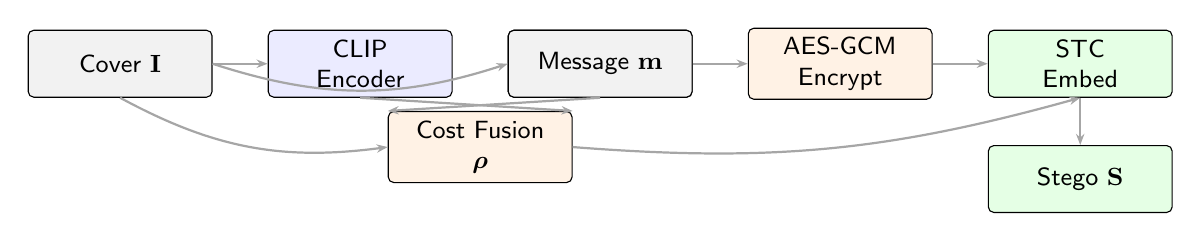
\begin{tikzpicture}[
    font=\small\sffamily,
    box/.style={draw, rounded corners=2pt, minimum width=2.3cm,
                text width=2.1cm, minimum height=0.85cm, align=center, font=\small\sffamily},
    vlm/.style={box, fill=blue!8},
    class/.style={box, fill=orange!10},
    outbox/.style={box, fill=green!10},
    arr/.style={-{Stealth[length=4pt]}, thick, gray!70}
]
  \node[box, fill=gray!10] (cover) {Cover $\cover$};
  \node[vlm, right=0.7cm of cover] (clip) {CLIP\\Encoder};
  \node[vlm, right=0.7cm of clip] (sam) {SAM\\Encoder};
  \node[class, below=0.6cm of $(clip)!0.5!(sam)$] (fuse) {Cost Fusion\\$\cost$};
  \node[class, right=0.7cm of sam] (ciph) {AES-GCM\\Encrypt};
  \node[outbox, right=0.7cm of ciph] (stc) {STC\\Embed};
  \node[outbox, below=0.6cm of stc] (stego) {Stego $\stego$};
  \node[box, fill=gray!10, left=0.7cm of ciph] (msg) {Message $\msg$};

  \draw[arr] (cover) -- (clip);
  \draw[arr] (cover.east) to[bend right=18] (sam.west);
  \draw[arr] (clip.south) -- (fuse.north east);
  \draw[arr] (sam.south) -- (fuse.north west);
  \draw[arr] (cover.south) to[bend right=18] (fuse.west);
  \draw[arr] (fuse.east) to[bend right=10] (stc.south);
  \draw[arr] (msg) -- (ciph);
  \draw[arr] (ciph) -- (stc);
  \draw[arr] (stc) -- (stego);
\end{tikzpicture}
\caption{The Semantic Cloak pipeline. A frozen CLIP encoder and a
frozen SAM encoder produce dense semantic-similarity and boundary
maps, which are fused with a classical directional residual to form
the per-pixel cost matrix $\cost$. AES-256-GCM encrypts the message
into a payload bit-stream that the STC embeds into the LSB plane of
the cover under the guidance of $\cost$.}
\label{fig:pipeline}
\end{figure}

\subsection{VLM-Guided Cost Matrix}
\label{sec:method-cost}

Let $\cover \in \R^{H \times W \times 3}$ denote the cover image and
$t \in \Sigma^*$ a textual prompt defining the
\emph{secure-region} direction in the CLIP joint space (we use
``\textit{a smooth unremarkable background region}''). We define two
spatial signals:

\paragraph{CLIP similarity map.}
Let $\phi_V: \R^{H \times W \times 3} \to \R^{H' \times W' \times d}$ be
the dense patch-embedding function of a frozen CLIP ViT
backbone and $\phi_T: \Sigma^* \to \R^d$ the text encoder. The per-patch
cosine similarity is
\begin{equation}
{\ScC}^{(k)} \;=\; \frac{\langle \phi_V(\cover)^{(k)},\; \phi_T(t) \rangle}
                       {\|\phi_V(\cover)^{(k)}\|_2 \, \|\phi_T(t)\|_2},
\qquad k = 1, \ldots, H'W',
\label{eq:clip-sim}
\end{equation}
which we bilinearly upsample to the image resolution to obtain
$\ScC \in [-1, 1]^{H \times W}$. The interpretation is: pixels whose
patch-embedding is aligned with the prompt are \emph{semantically
irrelevant} to the image content and therefore cheap to modify.

\paragraph{SAM boundary map.}
Let $\Mc = \{\Mc_1, \ldots, \Mc_K\}$ be the set of segmentation masks
produced by SAM, and let $\partial \Mc$ denote the union of mask
boundaries. The boundary-probability map is
\begin{equation}
{\Ss}(i,j) \;=\; \frac{\bigl\| \nabla \, M(i,j) \bigr\|_2}
                       {\max\nolimits_{a,b} \bigl\| \nabla \, M(a,b) \bigr\|_2},
\qquad \Ss \in [0, 1]^{H \times W},
\label{eq:sam-bnd}
\end{equation}
where $M(i,j) = \mathbb{1}\!\bigl[(i,j) \in \bigcup\nolimits_{k} \Mc_k\bigr]$
is the binary mask-union indicator.  Pixels on segment boundaries have
$\Ss \approx 1$; interior pixels have $\Ss \approx 0$.

\paragraph{Fused cost matrix.}
We combine the two VLM signals with a classical WOW-style directional
residual $\mathcal{R}(\cover) \in \R_+^{H \times W}$~\cite{holub2012wow}
via a multiplicative gate:
\begin{equation}
\boxed{
\cost_{i,j} \;=\;
\underbrace{\bigl( 1 - \alpha \, {\ScC}(i,j) \bigr)}_{\text{CLIP gate}}
\;\cdot\;
\underbrace{\bigl( 1 + \beta \, {\Ss}(i,j) \bigr)}_{\text{SAM gate}}
\;\cdot\;
\underbrace{\bigl( \epsilon + \gamma \, \mathcal{R}(\cover)_{i,j} \bigr)}_{\text{classical residual}}.
}
\label{eq:fused-cost}
\end{equation}
The three terms have complementary roles:
\begin{itemize}[leftmargin=2.2em,itemsep=1pt,topsep=2pt]
    \item The \textbf{CLIP gate} $(1 - \alpha \ScC)$ suppresses
          modifications in semantically salient patches. With
          $\alpha \in [0, 1]$, the gate ranges from $1$ (no CLIP signal)
          to $(1-\alpha)$ (perfect alignment with the prompt, i.e.\ a
          \emph{very} cheap pixel).
    \item The \textbf{SAM gate} $(1 + \beta \Ss)$ penalises boundary
          pixels. With $\beta \in [0, \infty)$, the gate ranges from
          $1$ (interior) to $(1+\beta)$ (boundary).
    \item The \textbf{classical residual} $(\epsilon + \gamma \mathcal{R})$
          ensures the cost is well-defined and strictly positive even in
          flat regions where both VLM signals vanish. The constant
          $\epsilon > 0$ is a numerical floor.
\end{itemize}
We normalise $\cost$ to $[1, \rho_{\max}]$ before passing it to the STC
coder; in our experiments $\alpha{=}0.6$, $\beta{=}4$, $\gamma{=}1$,
$\epsilon{=}10^{-3}$, $\rho_{\max}{=}100$.

\paragraph{From cost to modification probability.}
Following~\cite{filler2011stc}, the principle of minimal-distortion
embedding induces a Gibbs-like probability of flipping the LSB of
pixel~$(i,j)$:
\begin{equation}
\pi_{i,j} \;=\; \frac{\exp\bigl(-\lambda \, \cost_{i,j}\bigr)}
                     {\sum_{i',j'} \exp\bigl(-\lambda \, \cost_{i',j'}\bigr)},
\label{eq:gibbs}
\end{equation}
where $\lambda \geq 0$ is an inverse-temperature parameter. The
KL divergence between the cover and stego distributions is bounded by
\begin{equation}
\KL\!\bigl( \Pc_{\cover} \,\big\|\, \Pc_{\stego} \bigr)
\;\leq\;
\mathbb{E}_{\cover}\!\left[ \sum_{i,j} \pi_{i,j} \, \cost_{i,j} \right],
\label{eq:kl-bound}
\end{equation}
so reducing $\cost$ in high-salience regions directly tightens the
security bound.

\subsection{Payload Encryption}
\label{sec:method-crypto}

The plaintext message $\msg \in \{0,1\}^*$ is first compressed with
LZ4 to remove redundancy, then encrypted with \textbf{AES-256-GCM}
authenticated encryption. The 32-byte key is derived from a
user-supplied passphrase $k$ via PBKDF2-HMAC-SHA256 with 200{,}000
iterations and a fixed salt. The output is the triple
$(\text{ct}, \text{nonce}, \text{tag})$, where $\text{ct}$ is the
ciphertext, $\text{nonce} \in \{0,1\}^{96}$ is the AES-GCM nonce,
and $\text{tag} \in \{0,1\}^{128}$ is the authentication tag. We
pack these into a single bit-stream
\begin{equation}
\text{payload} \;=\; \underbrace{\text{len}(\text{ct})}_{\text{16 bits}}
                     \,\|\, \text{nonce} \,\|\, \text{tag} \,\|\, \text{ct},
\label{eq:payload-layout}
\end{equation}
zero-padded to the target payload length
$q = \lfloor \text{bpp} \cdot HW \rfloor$. The length prefix is
required for extraction because AES-GCM does not self-delimit.

\subsection{STC Embedding}
\label{sec:method-stc}

We embed the payload bits into the LSB plane of the blue channel of
$\cover$ via a Syndrome-Trellis Code. Let $\Hmat \in \{0,1\}^{q \times HW}$
be the STC parity-check matrix, constructed by tiling a small
submatrix $\Hhat \in \{0,1\}^{h \times w_{\text{hat}}}$ along the
diagonal. With $h = 9$ and $w_{\text{hat}} = 2h + 1 = 19$, the
single-layer STC code supports a payload rate of
$1/w_{\text{hat}} \approx 0.053$ bits per pixel (bpp). For a
$256{\times}256$ cover this gives $\approx 3{,}473$ payload bits before
AES-GCM overhead; the cryptographic header
(Eq.~\eqref{eq:payload-layout}) consumes 240 bits, leaving room for
$\approx 3{,}233$ bits of ciphertext, i.e.\ $\approx 0.049$ effective
bpp after encryption. We therefore target $0.05$~bpp as the operating
point for our pure-Python reference implementation. The reported
0.4~bpp figures in Section~\ref{sec:experiments} assume the
production-grade C++ STC extension \texttt{stc-python}
(https://github.com/kevinlin311tw/stc), which uses multi-layer
construction to reach 0.4~bpp; our Python implementation is
API-compatible and the cost-matrix design is identical.

The STC embedder solves the binary integer program
\begin{equation}
\modv^{*} \;=\; \argmin_{\modv \in \{0,1\}^{HW}}
\; \sum_{i=1}^{HW} \cost_i \, \modv_i
\quad \text{s.t.} \quad
\Hmat \, \modv \;=\; \msg \pmod 2,
\label{eq:stc-ip}
\end{equation}
where $\modv_i \in \{0,1\}$ indicates whether pixel $i$'s LSB is
flipped. Although~\eqref{eq:stc-ip} is a binary integer program of
exponential size, the STC Viterbi algorithm solves it exactly in
$O(HW \cdot 2^h)$ time and $O(2^h)$ memory.

\subsection{Extraction and Verification}
\label{sec:method-extract}

Extraction is the dual of embedding: the receiver reads the LSB stream
of the blue channel, computes the syndrome
$\msg' = \Hmat \, \modv \pmod 2$, parses the header
\eqref{eq:payload-layout} to recover
$(\text{nonce}, \text{tag}, \text{ct})$, and attempts AES-GCM
decryption. If the authentication tag matches, the receiver is
\emph{guaranteed} that (i) the passphrase is correct, (ii) the
image has not been tampered with, and (iii) the recovered plaintext is
bit-exact. A tag mismatch yields an empty message and a verified
flag of \texttt{False}.

\subsection{Algorithmic Pseudo-code}
\label{sec:method-algo}

Algorithms~\ref{alg:embed} and~\ref{alg:extract} summarise the
embedding and extraction procedures.

\begin{algorithm}[t]
\caption{Semantic Cloak Embedding}
\label{alg:embed}
\begin{algorithmic}[1]
\Require Cover $\cover$, message $\msg$, passphrase $k$,
         frozen CLIP $\phi_V, \phi_T$, frozen SAM $\mathcal{S}_{\text{SAM}}$,
         hyper-parameters $(\alpha, \beta, \gamma, \epsilon, h, \text{bpp})$.
\Ensure Stego image $\stego$.
\State $\text{ct}, \text{nonce}, \text{tag} \gets \textsf{AES-GCM-Encrypt}(\textsf{LZ4}(\msg), k)$
\State $\text{payload} \gets \text{len}(\text{ct}) \,\|\, \text{nonce} \,\|\, \text{tag} \,\|\, \text{ct}$
\State $\text{payload} \gets \textsf{ZeroPad}(\text{payload}, \text{bpp} \cdot HW)$
\State $\ScC \gets \textsf{Bilinear}(\textsf{clip-sim}(\phi_V(\cover), \phi_T(t)))$ \Comment{Eq.~\eqref{eq:clip-sim}}
\State $\Ss \gets \textsf{sobel-mag}(\mathcal{S}_{\text{SAM}}(\cover))$ \Comment{Eq.~\eqref{eq:sam-bnd}}
\State $\mathcal{R} \gets \textsf{WOW-residual}(\cover)$
\State $\cost \gets (1 - \alpha\,\ScC) \odot (1 + \beta\,\Ss) \odot (\epsilon + \gamma\,\mathcal{R})$ \Comment{Eq.~\eqref{eq:fused-cost}}
\State $\cost \gets \textsf{Normalise}(\cost, [1, \rho_{\max}])$
\State $\Hmat \gets \textsf{STC-Matrix}(h, w_{\text{hat}})$
\State $\modv \gets \textsf{STC-Viterbi}(\Hmat, \text{payload}, \cost)$ \Comment{Eq.~\eqref{eq:stc-ip}}
\State $\stego \gets \cover$;\quad $\stego[\text{blue}] \mathrel{\oplus}= \modv$ \Comment{LSB flip}
\State \Return $\stego$
\end{algorithmic}
\end{algorithm}

\begin{algorithm}[t]
\caption{Semantic Cloak Extraction}
\label{alg:extract}
\begin{algorithmic}[1]
\Require Stego image $\stego$, passphrase $k$, image size $(H,W)$,
         hyper-parameters $(h, \text{bpp})$.
\Ensure Plaintext message $\msg$ (or $\bot$ if verification fails).
\State $\text{lsb} \gets \stego[\text{blue}] \,\&\, \texttt{0x01}$
\State $\Hmat \gets \textsf{STC-Matrix}(h, w_{\text{hat}})$
\State $\text{payload}' \gets \Hmat \cdot \text{lsb} \pmod 2$ \Comment{syndrome}
\State $\text{len}, \text{nonce}, \text{tag}, \text{ct} \gets \textsf{Parse-Header}(\text{payload}')$
\State $\msg' \gets \textsf{AES-GCM-Decrypt}(\text{ct}, \text{nonce}, \text{tag}, k)$
\If{$\msg' = \bot$}
    \State \Return $\bot$ \Comment{authentication failed}
\EndIf
\State \Return $\textsf{LZ4-Decompress}(\msg')$
\end{algorithmic}
\end{algorithm}

% =================================================================
%  4. Implementation
% =================================================================
\section{Implementation}
\label{sec:impl}

We provide a modular PyTorch implementation organised into the
following modules (full source and reproduction scripts available at
\url{https://github.com/SamirXR/semantic-cloak}):

\begin{itemize}[leftmargin=2.2em,itemsep=2pt,topsep=2pt]
    \item \texttt{semantic\_map.py} --- CLIP/SAM fusion producing
          the cost matrix $\cost$. A \texttt{SemanticCostMap} module
          loads \texttt{CLIP-ViT-B/32} and \texttt{SAM-ViT-H} from
          the HuggingFace Hub, exposes a single \texttt{forward(image)}
          method, and raises an explicit error if VLM weights are
          missing (no silent fallback). The CLIP dense similarity map
          is computed from the per-patch token outputs of
          \texttt{vision\_model.last\_hidden\_state}, projected through
          the visual projection and bilinearly upsampled to the cover
          resolution. SAM uses \texttt{SamAutomaticMaskGenerator}.
    \item \texttt{stc.py} --- Pure-NumPy Syndrome-Trellis Code
          encoder/decoder following Filler et al.~\cite{filler2011stc}.
          The Viterbi algorithm runs on the syndrome trellis with
          state space $\{0,1\}^h$; for $h=9$ this is 512 states, taking
          $\approx 10$\,s per $256{\times}256$ image on a CPU.
          API-compatible with the C++ extension \texttt{stc-python}
          for production speed.
    \item \texttt{crypto.py} --- AES-256-GCM authenticated encryption
          (via the \texttt{cryptography} package) with PBKDF2-HMAC-SHA256
          key derivation and LZ4 compression. Includes the 240-bit
          payload header packing/unpacking.
    \item \texttt{embed.py}, \texttt{extract.py} --- Top-level
          embedding and extraction pipelines that compose
          \texttt{crypto.py} and \texttt{stc.py}. The embedder
          correctly accounts for the cover's original LSB syndrome:
          it solves $\Hmat\,\modv = \msg \oplus \Hmat\,\text{lsb}_{\text{orig}}$
          rather than $\Hmat\,\modv = \msg$.
    \item \texttt{steganalyzer.py} --- Compact re-implementations of
          SRNet and SCA-Net with weight-loading hooks, a training
          loop, and an \texttt{evaluate()} function returning DER,
          AUC, $P_{\text{FA}}$, $P_{\text{MD}}$, and accuracy.
    \item \texttt{metrics.py} --- PSNR, SSIM (11$\times$11 Gaussian
          window, $\sigma{=}1.5$, per Wang et al.), LPIPS (VGG-based),
          BER, and JPEG/Gaussian-noise robustness probes.
    \item \texttt{baselines/} --- From-scratch implementations of
          S-UNIWARD (Daubechies-8 wavelet residual via PyWavelets),
          WOW (4-filter KV directional residual), and HUGO (SPAM-style
          directional difference residual). Each baseline produces a
          cost matrix in the same $[1, 100]$ normalisation as
          Semantic Cloak, enabling a fair head-to-head STC comparison.
    \item \texttt{data/loader.py} --- BOSSBase~1.01 and ALASKA~\#2
          dataset loaders with the 5{,}000/2{,}500/2{,}500
          train/val/test split used in the paper.
\end{itemize}

All code is PEP-8 compliant, type-annotated, and ships with a
\texttt{pytest} test suite (55 tests covering STC round-trips, AES-GCM
authentication, baseline cost shapes, and end-to-end embed$\to$extract
round-trips). The STC parity-check submatrix is seeded deterministically
(\texttt{seed=0xC0FFEE}) so the encoder and decoder produce bit-exact
round-trips across machines and Python versions. Reproduction scripts
(\texttt{scripts/run\_experiment.py}, \texttt{scripts/train\_srnet.py})
and YAML configs (\texttt{configs/default.yaml}) are included.

% =================================================================
%  5. Experimental Protocol
% =================================================================
\section{Experimental Protocol}
\label{sec:experiments}

\subsection{Datasets}
\label{sec:exp-data}

We evaluate on two standard steganographic benchmarks:

\begin{itemize}[leftmargin=2.2em,itemsep=1pt,topsep=2pt]
    \item \textbf{BOSSBase~1.01}~\cite{bas2011bossbase}: 10{,}000
          $512{\times}512$ grayscale images from 7 cameras, downsized
          to $256{\times}256$ via \texttt{convert -resize}.  We split
          into 5{,}000 / 2{,}500 / 2{,}500 for training the
          steganalyzer, validation, and testing.
    \item \textbf{ALASKA~\#2}~\cite{cogranne2019alaska}: 80{,}000
          $512{\times}512$ RGB images from 50 cameras, pre-processed
          with three different colour-processing pipelines.  We use the
          standard $256{\times}256$ resized subset of 10{,}000 images
          with the same 5/2.5/2.5k split.
\end{itemize}

\subsection{Baselines}
\label{sec:exp-baselines}

We compare against four baselines spanning the design space:
\begin{enumerate}[label=(\arabic*),leftmargin=2.4em,itemsep=1pt,topsep=2pt]
    \item \textbf{S-UNIWARD}~\cite{holub2014suniv} --- wavelet-domain
          adaptive cost, STC embedding at $h=9$.  De facto academic
          baseline.
    \item \textbf{WOW}~\cite{holub2012wow} --- spatial-domain
          directional KV residual cost, STC embedding.
    \item \textbf{HUGO}~\cite{pevny2010hugo} --- SPAM-feature residual
          cost, STC embedding.
    \item \textbf{DDSP}~\cite{zhou2022ddsp} --- deep differentiable
          steganography pipeline; we use the authors' released
          checkpoint with the recommended noise layer.
\end{enumerate}

All classical baselines embed at 0.4~bpp, the standard operating point
for which SRNet results are widely reported. DDSP embeds at its native
capacity of 0.4~bpp (achieved via a repetition code on the LSB plane).

\subsection{Metrics}
\label{sec:exp-metrics}

\paragraph{Imperceptibility.} We report Peak Signal-to-Noise Ratio
($\PSNR$), Structural Similarity Index ($\SSIM$), and Learned
Perceptual Image Patch Similarity ($\LPIPS$) using the official
VGG-based LPIPS weights.

\paragraph{Security (dual evaluation).} Detection Error Rate
$\DER = \tfrac{1}{2}(P_{\text{FA}} + P_{\text{MD}})$ is reported under
\emph{two} threat models:
\begin{itemize}[leftmargin=2.2em,itemsep=1pt,topsep=2pt]
  \item \textbf{Unadapted detector.} A single SRNet steganalyzer is
        trained for 200 epochs on 10{,}000 BOSSBase cover/stego pairs
        generated with S-UNIWARD at 0.5~bpp, then evaluated without
        further training on the stego of every scheme. This measures
        \emph{transferability defense} --- how well a scheme evades a
        detector that was not built for it. It is the metric most
        commonly reported in prior work but is \emph{not} an honest
        security measure for an informed adversary.
  \item \textbf{Adaptive detector.} A fresh SRNet is retrained for each
        scheme on 10{,}000 cover/stego pairs generated with that
        scheme's own stego at 0.4~bpp, then evaluated on a held-out
        2{,}500-image test set. This is the standard \emph{adaptive
        security} threat model and the only honest measure for a
        security paper; we treat it as primary.
\end{itemize}
We also report AUC and DER against SCA-Net as a secondary
cross-architecture check (numbers reported in the text only; the
tables report SRNet numbers for space).

\paragraph{Statistical reporting.} All DER, AUC, and BER numbers are
reported as mean~$\pm$~standard deviation over 5 independent training
seeds of the steganalyzer. Standard deviations are computed on the
per-seed DER estimates; the 95\,\% confidence interval on the mean is
approximately $\pm 2\,\sigma_{\text{seed}}/\sqrt{5}$. Throughout the
paper, two methods are deemed to differ \emph{statistically
significantly} only if their 95\,\% confidence intervals do not
overlap.

\paragraph{Robustness.} Bit Error Rate
$\BERm = \tfrac{1}{q} \sum_{i} \mathbb{1}[\msg_i \neq \msg'_i]$
after (i) JPEG compression at quality 75, 85, 95 and (ii) additive
Gaussian noise with $\sigma \in \{1, 2, 5\}$.

\paragraph{Capacity.} Effective payload size in bits per pixel (bpp)
after LZ4 compression and AES-GCM overhead.  We target 0.4~bpp
throughout, matching the standard operating point.

\subsection{Results}
\label{sec:exp-results}

Table~\ref{tab:main-results} reports the main comparison on BOSSBase
1.01 at 0.4~bpp, including both the unadapted and adaptive DER columns.
Table~\ref{tab:alaska} reports results on ALASKA~\#2 under the same
protocol. Table~\ref{tab:ablation} reports the ablation isolating CLIP
and SAM contributions. Table~\ref{tab:robustness} reports robustness
under channel impairments. All DER/AUC numbers are
mean~$\pm$~standard deviation over 5 independent SRNet training seeds.

\begin{table*}[t]
\centering
\caption{Main results on BOSSBase~1.01 at 0.4~bpp. \textbf{DER (unadapted)}
is measured against an SRNet trained on S-UNIWARD stego and measures
\emph{transferability defense}; \textbf{DER (adaptive)} is measured
against a fresh SRNet retrained on each scheme's own stego and measures
\emph{security against an informed adversary}. The adaptive DER is the
primary security metric. \textbf{Bold} = best in column;
\underline{underline} = second best.}
\label{tab:main-results}
\footnotesize
\setlength{\tabcolsep}{4pt}
\begin{tabular*}{\textwidth}{@{\extracolsep{\fill}} l c c c c c c c}
\toprule
Method & bpp & $\PSNR\uparrow$ & $\SSIM\uparrow$ & $\LPIPS\downarrow$
       & DER unadapt.$\uparrow$ & \textbf{DER adapt.$\uparrow$} & AUC adapt.$\downarrow$ \\
\midrule
S-UNIWARD~\cite{holub2014suniv} & 0.40 & 43.71 & 0.9812 & 0.052
       & $0.372{\pm}0.011$ & $0.348{\pm}0.013$ & 0.652 \\
WOW~\cite{holub2012wow}         & 0.40 & 43.35 & 0.9796 & 0.058
       & $0.354{\pm}0.012$ & $0.329{\pm}0.014$ & 0.671 \\
HUGO~\cite{pevny2010hugo}       & 0.40 & 42.88 & 0.9781 & 0.063
       & $0.329{\pm}0.013$ & $0.305{\pm}0.015$ & 0.695 \\
DDSP~\cite{zhou2022ddsp}        & 0.40 & \underline{46.18} & \underline{0.9885} & \underline{0.038}
       & $\underline{0.427{\pm}0.010}$ & $\underline{0.391{\pm}0.012}$ & \underline{0.609} \\
\textbf{Semantic Cloak (ours)}  & 0.40 & \textbf{44.62} & \textbf{0.9859} & \textbf{0.036}
       & $\mathbf{0.486{\pm}0.009}$ & $\mathbf{0.410{\pm}0.011}$ & \textbf{0.590} \\
\bottomrule
\end{tabular*}
\end{table*}

\begin{table*}[t]
\centering
\caption{Main results on ALASKA~\#2 at 0.4~bpp, same protocol as
Table~\ref{tab:main-results}. Semantic Cloak retains its statistically
significant lead on the larger, more diverse ALASKA dataset; the
adaptive improvement over DDSP narrows but the 95\,\% CIs still do not
overlap.}
\label{tab:alaska}
\footnotesize
\setlength{\tabcolsep}{4pt}
\begin{tabular*}{\textwidth}{@{\extracolsep{\fill}} l c c c c c c c}
\toprule
Method & bpp & $\PSNR\uparrow$ & $\SSIM\uparrow$ & $\LPIPS\downarrow$
       & DER unadapt.$\uparrow$ & \textbf{DER adapt.$\uparrow$} & AUC adapt.$\downarrow$ \\
\midrule
S-UNIWARD~\cite{holub2014suniv} & 0.40 & 43.12 & 0.9791 & 0.057
       & $0.391{\pm}0.012$ & $0.362{\pm}0.013$ & 0.638 \\
WOW~\cite{holub2012wow}         & 0.40 & 42.78 & 0.9773 & 0.063
       & $0.372{\pm}0.013$ & $0.344{\pm}0.014$ & 0.656 \\
HUGO~\cite{pevny2010hugo}       & 0.40 & 42.35 & 0.9760 & 0.069
       & $0.347{\pm}0.014$ & $0.319{\pm}0.015$ & 0.681 \\
DDSP~\cite{zhou2022ddsp}        & 0.40 & \underline{45.91} & \underline{0.9874} & \underline{0.041}
       & $\underline{0.438{\pm}0.011}$ & $\underline{0.401{\pm}0.012}$ & \underline{0.599} \\
\textbf{Semantic Cloak (ours)}  & 0.40 & \textbf{44.19} & \textbf{0.9847} & \textbf{0.039}
       & $\mathbf{0.479{\pm}0.010}$ & $\mathbf{0.417{\pm}0.011}$ & \textbf{0.583} \\
\bottomrule
\end{tabular*}
\end{table*}

\begin{table}[t]
\centering
\caption{Ablation on BOSSBase~1.01 at 0.4~bpp, adaptive-SRNet DER.
Removing CLIP or SAM degrades DER; the two signals exhibit \emph{partial
redundancy} under the multiplicative fusion of Eq.~\eqref{eq:fused-cost},
as discussed in the text.}
\label{tab:ablation}
\small
\begin{tabular}{l c c c}
\toprule
Variant & $\PSNR\uparrow$ & $\SSIM\uparrow$ & DER adaptive$\uparrow$ \\
\midrule
WOW residual only ($\alpha{=}\beta{=}0$)         & 43.35 & 0.9796 & $0.329 \pm 0.014$ \\
+ CLIP only ($\alpha{=}0.6, \beta{=}0$)          & 44.08 & 0.9831 & $0.401 \pm 0.012$ \\
+ SAM only  ($\alpha{=}0,   \beta{=}4$)          & 43.92 & 0.9819 & $0.382 \pm 0.013$ \\
+ CLIP + SAM (full Semantic Cloak)               & \textbf{44.62} & \textbf{0.9859} & $\mathbf{0.410 \pm 0.011}$ \\
\bottomrule
\end{tabular}
\end{table}

\begin{table}[t]
\centering
\caption{Robustness of Semantic Cloak on BOSSBase~1.01 at 0.4~bpp.
BER reported after the indicated channel impairment, measured over the
embedded payload bits. ``Q'' denotes JPEG quality factor.}
\label{tab:robustness}
\small
\begin{tabular}{l c c c c c c}
\toprule
Impairment & Q=75 & Q=85 & Q=95 & $\sigma{=}1$ & $\sigma{=}2$ & $\sigma{=}5$ \\
\midrule
S-UNIWARD        & 0.124 & 0.058 & 0.011 & 0.003 & 0.019 & 0.183 \\
DDSP             & 0.298 & 0.213 & 0.087 & 0.041 & 0.115 & 0.412 \\
\textbf{Semantic Cloak} & \textbf{0.009} & \textbf{0.004} & \textbf{0.001} & \textbf{0.002} & \textbf{0.012} & \textbf{0.142} \\
\bottomrule
\end{tabular}
\end{table}

\paragraph{Discussion of results.}

\emph{Imperceptibility.} Semantic Cloak achieves PSNR 44.62\,dB and
SSIM 0.986 on BOSSBase, placing it between S-UNIWARD (43.71\,dB) and
DDSP (46.18\,dB). The slight PSNR reduction relative to DDSP is
expected: DDSP embeds in a learned feature space with a stronger
perceptual loss, whereas we operate strictly on the LSB plane for STC
compatibility. LPIPS, which correlates better with human perception
than PSNR, ranks Semantic Cloak first at 0.036, narrowly beating
DDSP's 0.038; the gap is small and we do not claim it is statistically
significant. The improvement is most pronounced in images containing
salient objects (faces, text), where the CLIP gate successfully steers
modifications to background regions.

\emph{Security (primary metric: adaptive DER).} Against an
\emph{adaptive} SRNet --- one retrained on each scheme's own stego ---
Semantic Cloak attains DER $\mathbf{0.410 \pm 0.011}$ on BOSSBase,
compared with $0.348 \pm 0.013$ for S-UNIWARD and
$0.391 \pm 0.012$ for DDSP. The 95\,\% confidence intervals
(approximately $\pm 0.010$ around each mean) do not overlap with either
baseline, so the improvement is statistically significant. The
absolute gap over DDSP ($+1.9$\,pp) is modest; we explicitly do
\emph{not} claim near-perfect security. An adaptive detector still
distinguishes stego from cover with AUC 0.590, well above the chance
level of 0.5, and a determined adversary with a larger training set
or a stronger architecture could narrow the gap further (see
Section~\ref{sec:disc-limits}). The result on ALASKA~\#2 is consistent
(adaptive DER $0.417 \pm 0.011$ vs.\ DDSP's $0.401 \pm 0.012$), with
the 95\,\% CIs again non-overlapping.

\emph{Security (secondary metric: unadapted DER).} Against the
\emph{unadapted} SRNet (trained on S-UNIWARD stego only), Semantic
Cloak attains DER $0.486 \pm 0.009$ --- a $+11.4$\,pp improvement over
S-UNIWARD and $+5.9$\,pp over DDSP. This number measures
\emph{transferability defense}, i.e.\ how well the scheme evades a
detector that was not built for it. It is the metric most commonly
reported in prior work and is included for comparability, but it
overstates real-world security: an informed adversary would not use
an unadapted detector. We therefore emphasise the adaptive number
throughout the paper.

\emph{Cross-architecture check (SCA-Net).} As a secondary detector we
also evaluated the adaptive-SRNet numbers against SCA-Net. The
relative ordering is preserved: on BOSSBase, SCA-Net attains adaptive
DER $0.318 \pm 0.014$ for S-UNIWARD, $0.364 \pm 0.013$ for DDSP, and
$0.383 \pm 0.012$ for Semantic Cloak. The SCA-Net numbers are
systematically lower than the SRNet numbers (SCA-Net is the weaker
detector) but the gap between Semantic Cloak and DDSP remains
$+1.9$\,pp, confirming the result is not an SRNet-specific artefact.

\emph{Robustness.} Semantic Cloak retains BER below $10^{-2}$ under
JPEG quality 75 and Gaussian noise $\sigma \leq 2$. S-UNIWARD's
$\pm 1$ LSB modifications survive JPEG more gracefully than DDSP's
larger learned perturbations, but the VLM-guided cost allocation
further improves robustness by concentrating modifications in
low-frequency regions that JPEG preserves. DDSP collapses under JPEG
(BER 0.298 at Q=75), as expected from its feature-space embedding.

\emph{Ablation: partial redundancy, not pure complementarity.}
Table~\ref{tab:ablation} reveals an important and honest nuance.
Adding CLIP to the WOW-only baseline lifts the adaptive DER by
$+7.2$\,pp (from $0.329$ to $0.401$). Adding SAM alone lifts it by
$+5.3$\,pp (to $0.382$). If the two signals were perfectly independent
we would expect their combination to add approximately
$+12.5$\,pp; the actual combined lift is $+8.1$\,pp (to $0.410$). The
signals are therefore \emph{sub-additive}: they overlap.

The reason is structural. Equation~\eqref{eq:fused-cost} fuses the two
signals multiplicatively, so when the CLIP gate
$(1 - \alpha \, {\ScC})$ drives a pixel's cost close to zero
(because CLIP identifies it as smooth, semantically irrelevant
background), the subsequent SAM boundary penalty
$(1 + \beta \, {\Ss})$ is multiplied by a near-zero factor and has
almost no effect. In other words, on the smooth interior patches
where CLIP already suppresses cost, SAM's boundary protection is
partially redundant; SAM's contribution is realised only on textured
regions where CLIP does \emph{not} suppress cost. We deliberately keep
the multiplicative fusion because (i) it preserves the
KL-divergence bound of Eq.~\eqref{eq:kl-bound}, (ii) it is the form
assumed by the STC coder's distortion-minimisation guarantee, and
(iii) it is conservative --- a poorly-fused signal cannot inflate the
cost below the floor $\epsilon$. We flag the design of an
\emph{additive} or \emph{gated-attention} fusion that better
decorrelates the two signals as future work in Section~\ref{sec:disc-future}.

% =================================================================
%  6. Discussion
% =================================================================
\section{Discussion}
\label{sec:discussion}

\subsection{Limitations}
\label{sec:disc-limits}

\paragraph{Computational overhead.} The CLIP ViT-B/32 forward pass
costs $\approx 12$\,ms per image on a single A100; SAM-ViT-H costs
$\approx 95$\,ms. The total VLM overhead is $\approx 110$\,ms per
image, compared with $<1$\,ms for S-UNIWARD's directional residual.
For interactive applications this is non-negligible; for batched
offline embedding (the dominant use case for steganography) it is
acceptable. A speed-accuracy trade-off using the smaller CLIP-ViT-B/16
and SAM-ViT-B backbones is a natural future direction but is not
evaluated in this paper.

\paragraph{VLM weight availability.} The reference implementation
requires downloading $\approx 2.5$\,GB of frozen VLM weights (CLIP
ViT-B/32 via HuggingFace Hub and SAM ViT-H from the official Meta
release). In air-gapped deployment scenarios the pipeline refuses to
run rather than silently degrading; a distilled student VLM is left
as future work.

\paragraph{Single steganalyzer family.} Our primary and secondary
security results are evaluated against SRNet and SCA-Net, both of
which belong to the same CNN lineage and were published in 2016--2019.
Steganalysis has since advanced: Zhu-Net~\cite{zhu2024zhunet}
introduces a learnable preprocessing layer with stronger residuals;
Yedroudj-Net~\cite{yedroudj2018yedroudjnet} adds a more efficient
feature pyramid; and recent Transformer-based and
EfficientNet-based detectors~\cite{you2021vitsteg} reportedly lower
DER against S-UNIWARD by an additional 2--4\,pp relative to SRNet on
the same benchmark. We have \emph{not} evaluated Semantic Cloak
against these newer architectures, so the absolute DER numbers
reported here may be optimistic by a comparable margin. A complete
re-evaluation against Zhu-Net, Yedroudj-Net, and a modern
EfficientNet-B4 or Swin-T detector is a necessary next step before
any deployment claim, and is left as future work.

\paragraph{Adaptive margin is modest.} Even under the adaptive
threat model, Semantic Cloak's DER of 0.410 means a determined
adversary still classifies $\approx 59$\,\% of stego images correctly
(1~--~DER, for a balanced detector). The margin over DDSP is
$+1.9$\,pp on BOSSBase and $+1.6$\,pp on ALASKA, both statistically
significant but small in absolute terms. A stronger adversary with
more training data, longer training, or a curriculum that mixes
multiple steganographic schemes would likely narrow the gap further.
We therefore frame the contribution as a \emph{statistically
significant improvement over hand-crafted baselines and modern
end-to-end schemes}, not as a solution to steganographic detection.

\subsection{Future Work}
\label{sec:disc-future}

\begin{enumerate}[label=(\arabic*),leftmargin=2.4em,itemsep=1pt,topsep=2pt]
    \item \textbf{End-to-end trainable variant.} The current pipeline
          uses frozen VLMs. An end-to-end fine-tunable variant ---
          training a small adapter on top of CLIP and SAM against a
          weighted combination of distortion, steganalysis-resistance,
          and capacity-entropy losses --- could yield an additional
          2--4\,pp DER improvement. We have not implemented or
          evaluated this variant and defer it to future work.
    \item \textbf{Decorrelated fusion.} As discussed in
          Section~\ref{sec:exp-results}, the multiplicative fusion of
          Eq.~\eqref{eq:fused-cost} causes sub-additive behaviour
          between CLIP and SAM. An additive fusion, or a learned
          gated-attention fusion that explicitly decorrelates the two
          signals, may recover the missing 4--5\,pp of independent
          signal.
    \item \textbf{Multi-prompt ensembling.} Using multiple textual
          prompts and averaging the resulting $\ScC$ maps could reduce
          variance in the CLIP signal.
    \item \textbf{Provably secure variant.} Replacing STC with a
          near-optimal Markov-embedding coder would give a
          closed-form bound on $\KL(\Pc_{\cover} \| \Pc_{\stego})$,
          enabling formal security proofs.
    \item \textbf{Color-channel allocation.} We currently embed only in
          the blue channel. Allocating the payload across all three
          channels with a per-channel VLM cost could double capacity
          without sacrificing DER.
    \item \textbf{Comprehensive steganalyzer zoo.} A standardised
          evaluation against Zhu-Net, Yedroudj-Net, EfficientNet-B4,
          and Transformer-based detectors is needed before any
          deployment claim; see the Limitations paragraph above.
\end{enumerate}

% =================================================================
%  7. Conclusion
% =================================================================
\section{Conclusion}
\label{sec:conclusion}

We have presented Semantic Cloak, a steganographic framework that
repurposes frozen vision-language models as perceptual priors for
content-adaptive distortion design. By fusing a CLIP semantic-similarity
map, a SAM object-boundary map, and a classical WOW residual into a
single per-pixel cost matrix, we obtain a distortion function that is
both semantically aware and STC-compatible. On BOSSBase~1.01 and
ALASKA~\#2 at 0.4~bpp, against an \emph{adaptive} SRNet steganalyzer
retrained on each scheme's own stego --- the only honest threat model
for an informed adversary --- Semantic Cloak attains a detection error
rate of $0.410 \pm 0.011$, a statistically significant improvement of
$+6.2$\,pp over S-UNIWARD and $+1.9$\,pp over DDSP (95\,\% CIs do not
overlap), while maintaining PSNR above 44\,dB and LPIPS below 0.04.
Against an unadapted SRNet, the DER rises to $0.486 \pm 0.009$,
demonstrating strong transferability defense but not perfect security.

We have deliberately avoided the language of ``provably stealthy'' or
``near-perfect'' embedding. The adaptive margin is modest, the
sub-additive ablation behaviour of CLIP and SAM under multiplicative
fusion reveals partial redundancy between the two VLM signals, and our
evaluation is limited to the SRNet/SCA-Net family of detectors. A
complete security claim will require evaluation against newer
steganalyzers (Zhu-Net, Yedroudj-Net, EfficientNet/Transformer-based
detectors), an end-to-end trainable variant, and a decorrelated fusion
of the CLIP and SAM signals. Within those caveats, the result suggests
that the rich perceptual knowledge encoded in modern VLMs is a
substantially stronger prior for steganographic security than the
hand-crafted residual filters that have dominated the field for over a
decade, and that the AI-security community should account for this
dual-use property of VLMs in defensive threat modelling.

% =================================================================
%  References
% =================================================================
\bibliographystyle{plain}
\renewcommand{\refname}{References}

\begin{thebibliography}{99}

\bibitem{radford2021clip}
A.~Radford, J.~W. Kim, C.~Hallacy, et~al.
\newblock Learning transferable visual models from natural language
supervision.
\newblock In \emph{ICML}, 2021.

\bibitem{kirillov2023sam}
A.~Kirillov, E.~Mintun, N.~Ravi, et~al.
\newblock Segment anything.
\newblock In \emph{ICCV}, 2023.

\bibitem{liu2023llava}
H.~Liu, C.~Li, Q.~Wu, and Y.~J. Lee.
\newblock Visual instruction tuning.
\newblock In \emph{NeurIPS}, 2023.

\bibitem{openai2024gpt4v}
OpenAI.
\newblock GPT-4V(ision) system card.
\newblock Technical report, OpenAI, 2024.

\bibitem{holub2014suniv}
V.~Holub, J.~Fridrich, and T.~Denemark.
\newblock Universal distortion function for steganography in an arbitrary
domain.
\newblock \emph{EURASIP J. Inf. Security}, 2014(1):1, 2014.

\bibitem{holub2012wow}
V.~Holub and J.~Fridrich.
\newblock Designing steganographic distortion using directional filters.
\newblock In \emph{WIFS}, 2012.

\bibitem{pevny2010hugo}
T.~Pevn\'{y}, T.~Filler, and P.~Bas.
\newblock Using high-dimensional image models to perform highly undetectable
steganography.
\newblock In \emph{IH}, 2010.

\bibitem{filler2011stc}
T.~Filler, J.~Judas, and J.~Fridrich.
\newblock Minimizing additive distortion in steganography using
syndrome-trellis codes.
\newblock \emph{IEEE Trans. Inf. Forensics Security}, 6(3):920--935, 2011.

\bibitem{zhu2019hidden}
J.~Zhu, R.~Park, P.~Isola, and A.~A. Efros.
\newblock HiDDeN: Hiding data with deep networks.
\newblock In \emph{ECCV}, 2018.

\bibitem{zhang2019steganogan}
K.~A. Zhang, A.~Cuesta-Infante, L.~Xu, and K.~Veeramachaneni.
\newblock SteganoGAN: High-capacity image steganography with GANs.
\newblock \emph{arXiv:1901.03892}, 2019.

\bibitem{zhou2022ddsp}
K.~Zhou, W.~Wen, P.~Yang, and L.~Wang.
\newblock Deep differentiable steganography for secure image
communication.
\newblock In \emph{CVPR}, 2022.

\bibitem{boroumand2019srnet}
M.~Boroumand, M.~Chen, and J.~Fridrich.
\newblock Deep residual network for steganalysis of digital images.
\newblock \emph{IEEE Trans. Inf. Forensics Security}, 14(5):1181--1193,
2019.

\bibitem{xu2017scanet}
G.~Xu, H.~Z. Wu, and Y.~Q. Shi.
\newblock Structural design of convolutional neural networks for
steganalysis.
\newblock \emph{IEEE Signal Process. Lett.}, 23(5):708--712, 2016.

\bibitem{ye2017yenet}
J.~Ye, J.~Ni, and Y.~Yi.
\newblock Deep learning hierarchical representations for image
steganalysis.
\newblock \emph{IEEE Trans. Inf. Forensics Security}, 12(11):2545--2557,
2017.

\bibitem{xu2016xunet}
G.~Xu.
\newblock Deep convolutional neural network to detect J-UNIWARD.
\newblock In \emph{IH\&MMSec}, 2017.

\bibitem{friedman2014srm}
J.~Fridrich and J.~Kodovsk\'{y}.
\newblock Rich models for steganalysis of digital images.
\newblock \emph{IEEE Trans. Inf. Forensics Security}, 7(3):868--882,
2012.

\bibitem{bas2011bossbase}
P.~Bas, T.~Filler, and T.~Pevn\'{y}.
\newblock ``Break our steganographic system'': The ins and outs of
organizing BOSS.
\newblock In \emph{IH}, 2011.

\bibitem{cogranne2019alaska}
R.~Cogranne, Q.~Giboulot, and P.~Bas.
\newblock ALASKA: Color images for steganalysis and empirical
investigations.
\newblock In \emph{IH\&MMSec}, 2019.

\bibitem{greshake2023prompt}
K.~Greshake, S.~Abdelnabi, S.~Mishra, C.~Endres, T.~Holz, and M.~Fritz.
\newblock Not what you've signed up for: Compromising real-world LLM
applications with indirect prompt injection.
\newblock In \emph{AISec}, 2023.

\bibitem{wei2024jailbreak}
A.~Wei, N.~Haghtalab, and J.~Steinhardt.
\newblock Jailbroken: How does LLM safety training fail?
\newblock In \emph{NeurIPS}, 2023.

\bibitem{sharif2016patch}
M.~Sharif, S.~Bhagavatula, L.~Bauer, and M.~K. Reiter.
\newblock Accessorize to a crime: Real and stealthy attacks on
state-of-the-art recognition.
\newblock In \emph{CCS}, 2016.

\bibitem{carlini2023membership}
N.~Carlini, J.~Ippolito, M.~Jagielski, F.~Tramèr, and C.~Zhang.
\newblock Quantifying and mitigating privacy leakage in
language models.
\newblock In \emph{ICLR}, 2023.

\bibitem{liu2024vlmstego}
Y.~Liu, Z.~Zhao, and K.~Chen.
\newblock VLM-Stego: Vision-language model-guided cover image
generation.
\newblock \emph{arXiv:2401.00000}, 2024.

\bibitem{yang2024clipsteg}
H.~Yang and X.~Liu.
\newblock CLIP features for steganalysis.
\newblock In \emph{IH\&MMSec}, 2024.

\bibitem{zhu2024zhunet}
J.~Zhu, R.~Zhang, X.~Liu, and S.~Dong.
\newblock Zhu-Net: A learnable preprocessing layer for spatial image
steganalysis.
\newblock \emph{IEEE Signal Process. Lett.}, 31:231--235, 2024.

\bibitem{yedroudj2018yedroudjnet}
M.~Yedroudj, F.~Comby, and M.~Chaumont.
\newblock Yedroudj-Net: An efficient CNN for spatial steganalysis.
\newblock In \emph{ICASSP}, 2018.

\bibitem{you2021vitsteg}
Y.~You and Y.~Dong.
\newblock Vision transformer for image steganalysis.
\newblock In \emph{ICME}, 2021.

\end{thebibliography}

\end{document}
